\section{Risultati Ottenuti}

I risultati ottenuti, che verranno analizzati in dettaglio nelle 
sezioni successive, possono essere riassunti in termini generali come 
risultati positivi, sia in termini di prestazioni del modello che di 
efficacia delle politiche di intervento adottate. In particolare, 
è evidente che il tempo totale di simulazione è principalmente 
influenzato dall'implementazione del controllore e, di conseguenza, 
dal calcolo delle Neural ODE e da tutte le operazioni connesse.

\begin{table}[htb]
    \centering
    \caption{Benchmarking con BenchmarkTools.jl \cite{chen2016robust}}
    \begin{tabular}{|p{2.57cm}||p{2.57cm}|p{2.57cm}|p{2.57cm}|p{2.57cm}|}
        \hline
        \multicolumn{5}{|c|}{Singlerun} \\
        \hline
        & Nessun Intervento & Intervento Non Farmaceutico & Intervento Farmaceutico & Intervento Farmaceutico e Non \\
        \hline
        Evaluation Time & 11.12 s & 1004.52 s & 12.28 s & 883.85 s \\
        GC Time & 6.09\% GC & 11.03\% GC & 6.56\% GC & 10.77\% GC \\
		Memory Estimation & 6.13 GiB & 1.05 TiB & 7.93 GiB & 936.06 GiB \\
        \# Allocation & 80299055 & 11803509066 & 88006856 & 10487571414 \\
		\hline
    \end{tabular}
\end{table}

I lunghi tempi di calcolo riscontrati sono principalmente attribuibili 
al processo di calcolo delle contromisure non farmaceutiche applicate 
alla popolazione. Diversamente, le contromisure farmaceutiche, 
se applicate con tempismo adeguato, oltre a contribuire in modo 
significativo alla riduzione della diffusione della pandemia 
(vedi Figura \ref{fig:comparison_vax_1}, Figura 
\ref{fig:comparison_vax_2}, Figura \ref{fig:comparison_vax_3}, 
Figura \ref{fig:comparison_vax_4}), consentono anche una significativa 
riduzione dei tempi di calcolo.

\begin{table}[htb]
    \centering
    \caption{Risultati Ensemblerun con ProgressMeter.jl}
    \begin{tabular}{|p{2.57cm}||p{2.57cm}|p{2.57cm}|p{2.57cm}|p{2.57cm}|}
        \hline
        \multicolumn{5}{|c|}{Singlerun} \\
        \hline
        & Nessun Intervento & Intervento Non Farmaceutico & Intervento Farmaceutico & Intervento Farmaceutico e Non \\
        \hline
        5 Run (Progress: 100\%) H:MM:SS & Time: 0:00:56 & Time: 1:21:33 & Time: 0:01:06 & Time: 1:09:45 \\
        \hline
    \end{tabular}
\end{table}

In altre parole, l'applicazione tempestiva di misure farmaceutiche, 
come la somministrazione di vaccini, non solo contribuisce in modo 
sostanziale a mitigare la diffusione del virus, ma riduce anche 
sensibilmente i tempi necessari per completare le simulazioni. 
Questo aspetto sottolinea l'importanza delle strategie di vaccinazione 
e delle misure farmaceutiche nella gestione delle pandemie, 
non solo dal punto di vista della salute pubblica, ma anche dal punto 
di vista della computazione e dell'efficienza dei modelli epidemiologici.
\newpage

\subsection{Nessun Intervento}

Il seguente grafico (Figura \ref{fig:abm_no_intervent}) mostra 
l'andamento delle curve del modello quando questo viene eseguito 
senza alcuna tipologia di intervento. Questo andamento è rappresentato 
in modo cumulativo rispetto all'andamento dei singoli agenti, 
i quali possono mostrare comportamenti differenti tra loro.

\begin{minipage}{\linewidth}
    \centering
    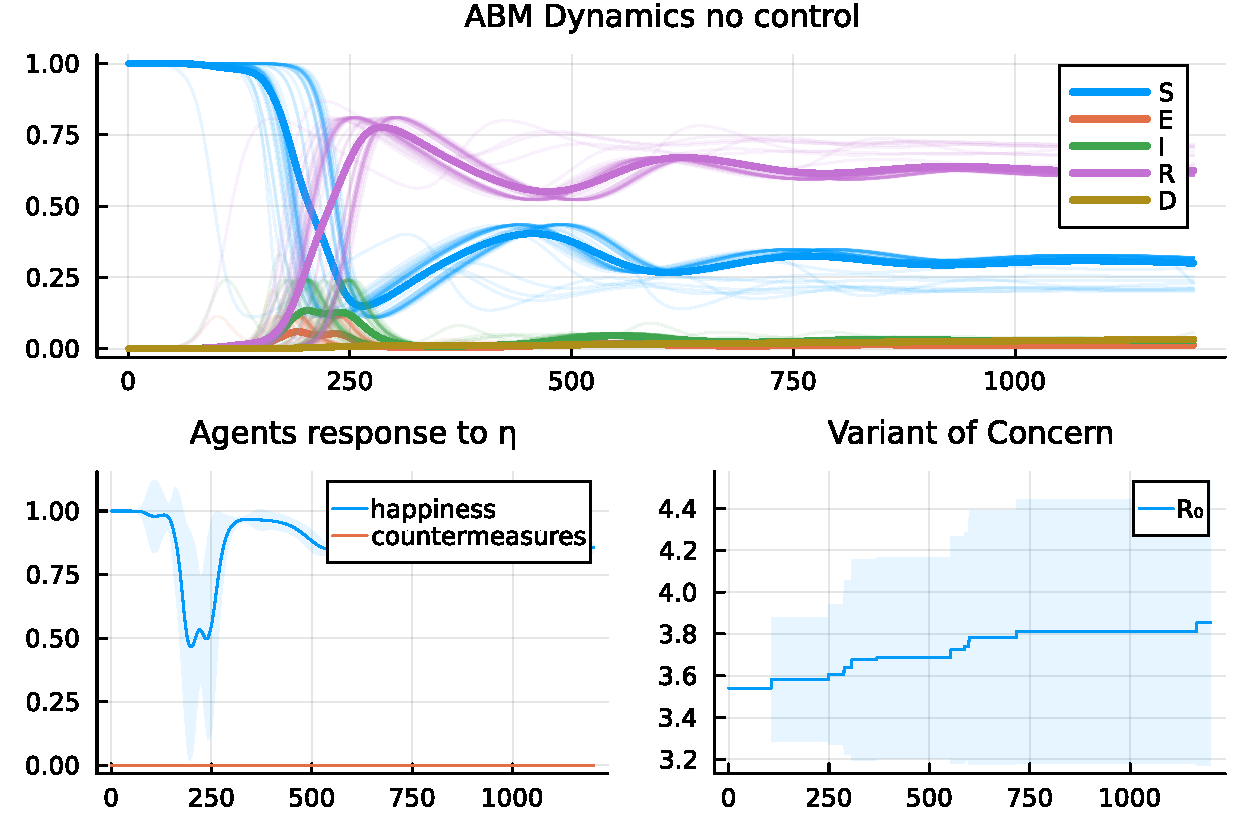
\includegraphics[width=\textwidth]{img/SocialNetworkABM_NO_CONTROL.pdf}
    \captionof{figure}{Grafico cumulativo del modello senza alcun tipo di intervento}
    \label{fig:abm_no_intervent}
\end{minipage}

Complessivamente, l'andamento del modello è simile a quello 
standard di un modello di tipo SEIR, con alcune variazioni 
dovute ai fattori di stocasticità intrinseci del modello. 
Il grafico mostra le traiettorie più comuni delle curve cumulative 
del modello, mettendo in evidenza i percorsi più frequenti.

Come è possibile notare, il numero di individui suscettibili 
diminuisce drasticamente a causa della rapida diffusione 
esponenziale del virus. Questo è accompagnato da una crescita 
altrettanto rapida del numero di individui guariti (recovered). 
Tuttavia, a causa della definizione delle condizioni per i guariti, 
questi individui non sono immuni alle varianti del virus, il che 
permette di modellare una possibile ciclicità dell'epidemia 
dovuta alla perdita di immunità della popolazione. 
Queste proprietà contribuiscono all'andamento ciclico delle curve. 
Inoltre, si nota che la curva associata all'andamento degli 
individui nella classe \emph{D} ha una crescita lineare, 
sebbene non molto evidente.

La curva associata alla variabile di "happiness" del modello, 
utilizzata per bilanciare la severità delle misure di controllo 
per evitare un ciclo insostenibile, mostra un comportamento 
piuttosto peculiare. Questo è principalmente dovuto alla 
definizione della funzione di controllo della felicità 
(vedi Figura \ref{fig:happinessf}). Inoltre, la curva tende 
ad oscillare in modo ciclico a causa della definizione delle 
misure di controllo.

In generale, il modello senza interventi mostra un'epidemia in 
rapida crescita seguita da periodi ciclici di riduzione della 
diffusione del virus.

\subsection{Intervento Non Farmaceutico}

Nel seguente grafico (Figura \ref{fig:abm_nonpharm_intervent}) è 
rappresentato l'andamento delle curve quando viene applicato un 
intervento non farmaceutico, come il distanziamento sociale, 
l'uso di maschere, ecc. L'obiettivo di questo tipo di intervento 
è quello di rallentare la diffusione del virus senza utilizzare 
farmaci o vaccini.

\begin{minipage}{\linewidth}
    \centering
    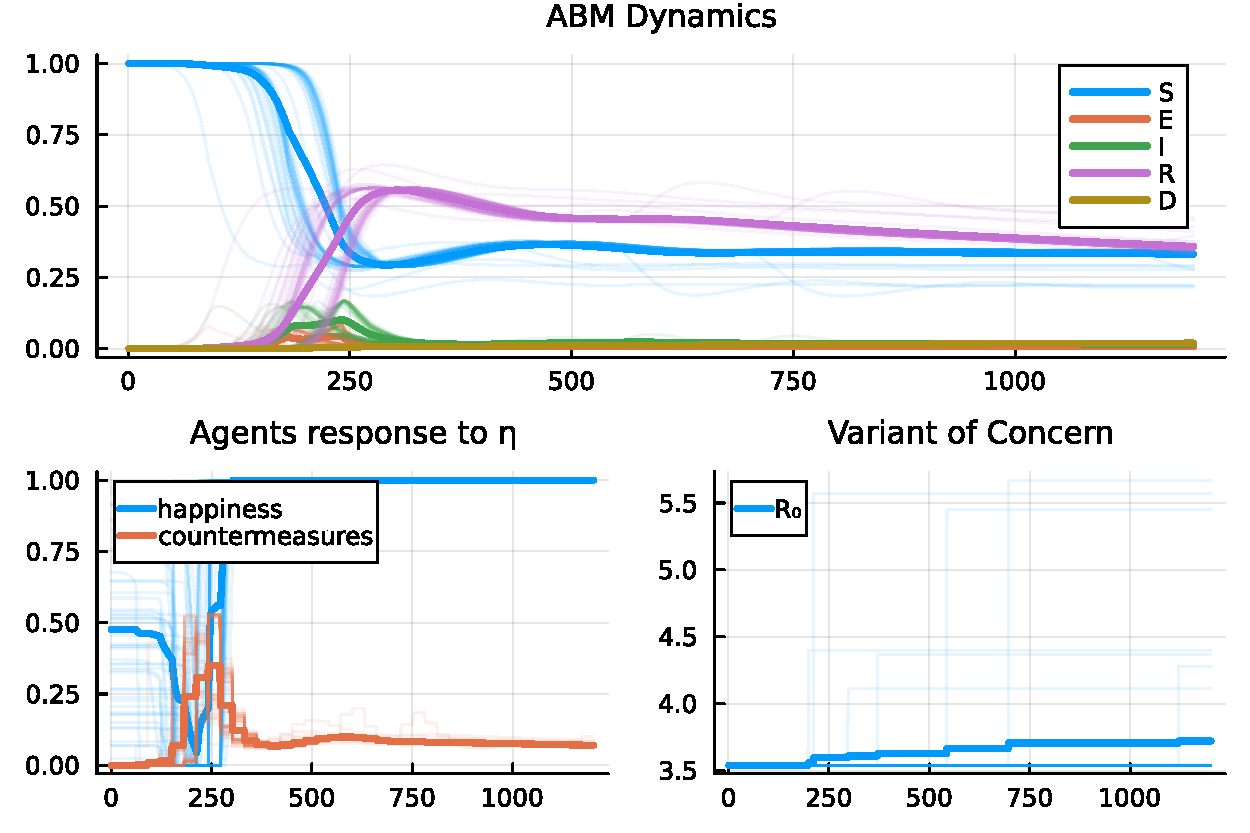
\includegraphics[width=\textwidth]{img/SocialNetworkABM_CONTROL.pdf}
    \captionof{figure}{Grafico cumulativo del modello con intervento non farmaceutico}
    \label{fig:abm_nonpharm_intervent}
\end{minipage}

Come si può vedere dal grafico, l'intervento non farmaceutico 
ha un impatto significativo sulla diffusione del virus. 
In particolare, il numero di individui suscettibili rimane 
più stabile nel tempo rispetto al caso senza interventi, e il 
picco dell'epidemia è notevolmente ridotto. Questo è dovuto 
all'efficacia delle misure di distanziamento sociale e al fatto 
che esse riducono il tasso di contatto tra gli individui infetti 
e suscettibili. Tuttavia, il numero di individui guariti è ancora 
ciclico a causa della perdita di immunità, e la curva di felicità 
mostra comunque oscillazioni dovute alle misure di controllo cicliche.

In generale, l'intervento non farmaceutico riesce a contenere 
l'epidemia e a ridurne l'entità, ma non riesce a eliminarla 
completamente.

\subsection{Intervento Farmaceutico}

Il seguente grafico (Figura \ref{fig:abm_pharm_intervent}) 
rappresenta l'andamento delle curve quando viene applicato un 
intervento farmaceutico, come la somministrazione di vaccini o 
farmaci antivirali. L'obiettivo di questo tipo di intervento è 
quello di ridurre significativamente la diffusione del virus e, 
idealmente, di eliminare l'epidemia.

\begin{minipage}{\linewidth}
    \centering
    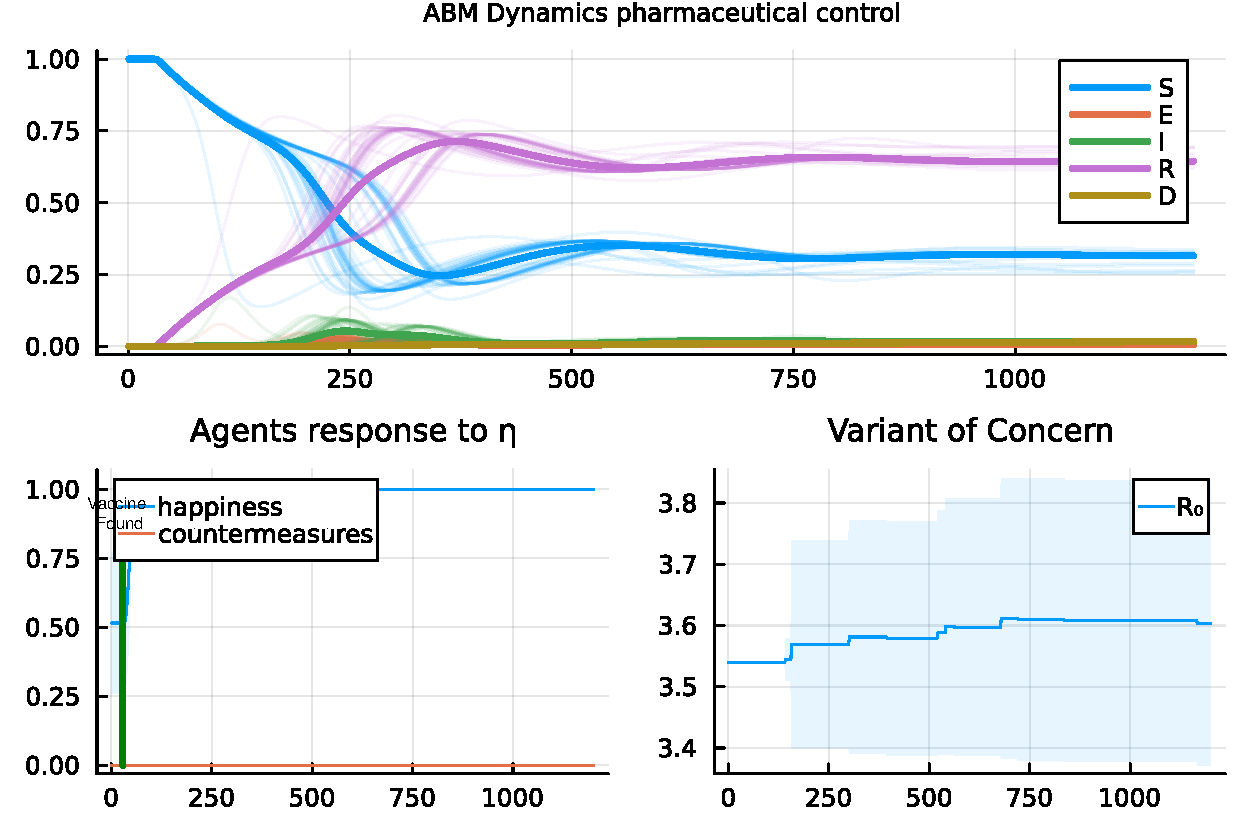
\includegraphics[width=\textwidth]{img/SocialNetworkABM_VACCINE.pdf}
    \captionof{figure}{Grafico cumulativo del modello con intervento farmaceutico}
    \label{fig:abm_pharm_intervent}
\end{minipage}

Come si può notare, l'intervento farmaceutico ha un impatto 
molto positivo sulla diffusione del virus. Il numero di individui 
suscettibili rimane stabile nel tempo, e l'epidemia viene rapidamente 
contenuta. Questo è dovuto alla somministrazione di farmaci o vaccini, 
che riducono la capacità di trasmissione del virus e proteggono gli 
individui suscettibili. Inoltre, il numero di individui guariti non 
mostra più l'andamento ciclico, poiché i soggetti guariti attraverso 
l'intervento farmaceutico acquisiscono immunità duratura.

La curva di felicità mostra ancora alcune oscillazioni dovute alle 
misure di controllo cicliche, ma queste oscillazioni sono meno 
pronunciate rispetto ai casi precedenti.

In generale, l'intervento farmaceutico è estremamente efficace nel 
contenere e ridurre l'epidemia.

\subsubsection{Grafici di Confronto}

I grafici di confronto mostrano l'impatto del momento di inizio della 
campagna di vaccinazione su diversi scenari. Questi grafici illustrano 
come l'efficacia della campagna vaccinale possa dipendere dal suo avvio, 
oltre al numero di persone vaccinate.

\begin{figure}[!hb]
	\centering
	\begin{subfigure}[b]{0.45\textwidth}
		\centering
		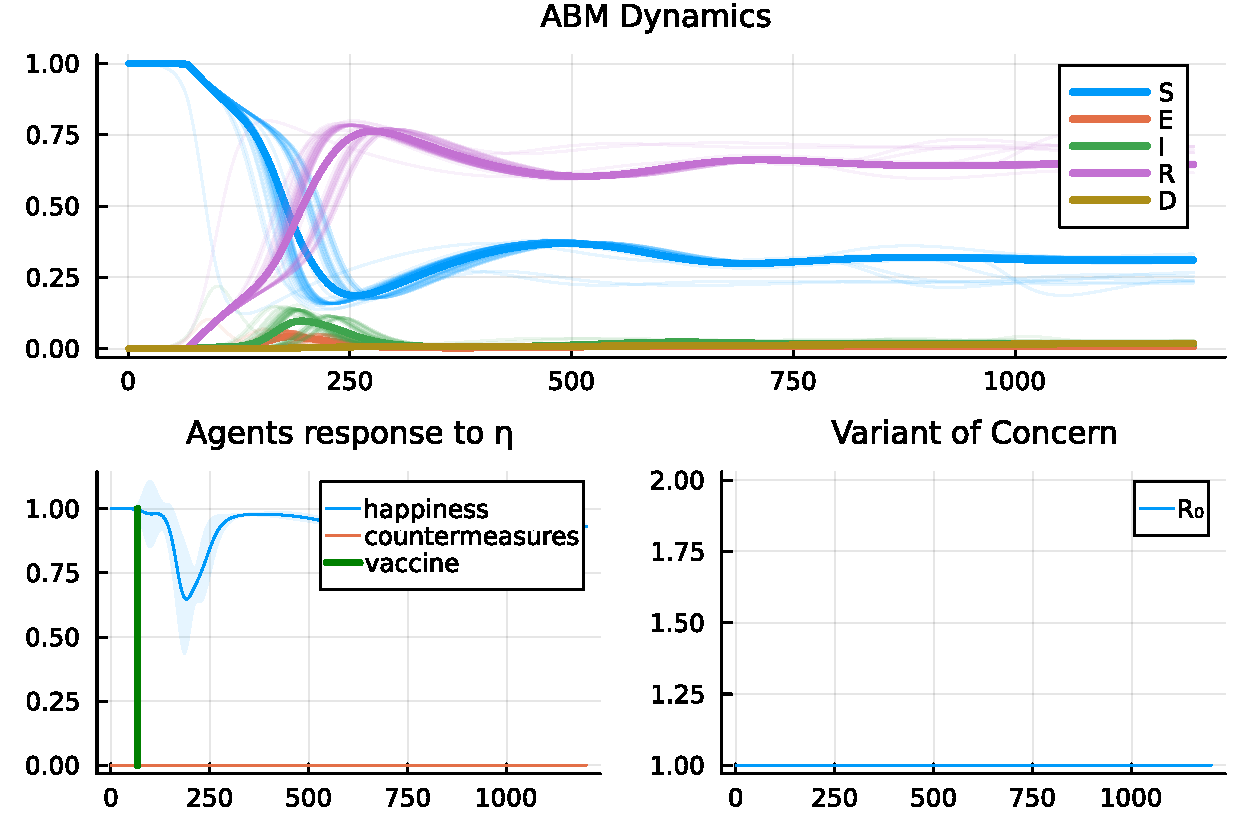
\includegraphics[width=\textwidth]{img/SocialNetworkABM_1_V.pdf}
		\caption{Grafico per la comparazione sul periodo di inizio della campagna vaccinale. Immediata}
		\label{fig:comparison_vax_1}
	\end{subfigure}
	\hfill
	\begin{subfigure}[b]{0.45\textwidth}
		\centering
		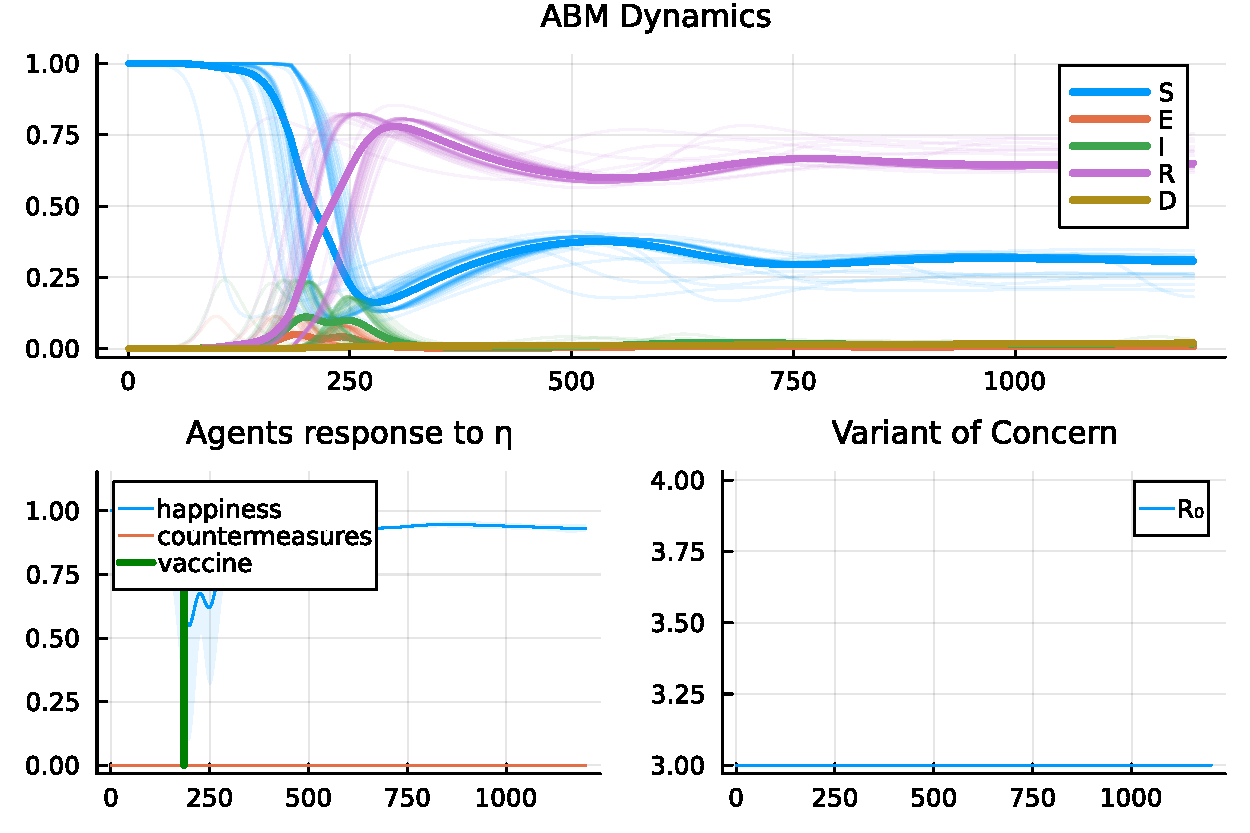
\includegraphics[width=\textwidth]{img/SocialNetworkABM_3_V.pdf}
		\caption{Grafico per la comparazione sul periodo di inizio della campagna vaccinale. Durante prima ondata}
		\label{fig:comparison_vax_2}
	\end{subfigure}
	\hfill
	\begin{subfigure}[b]{0.45\textwidth}
		\centering
		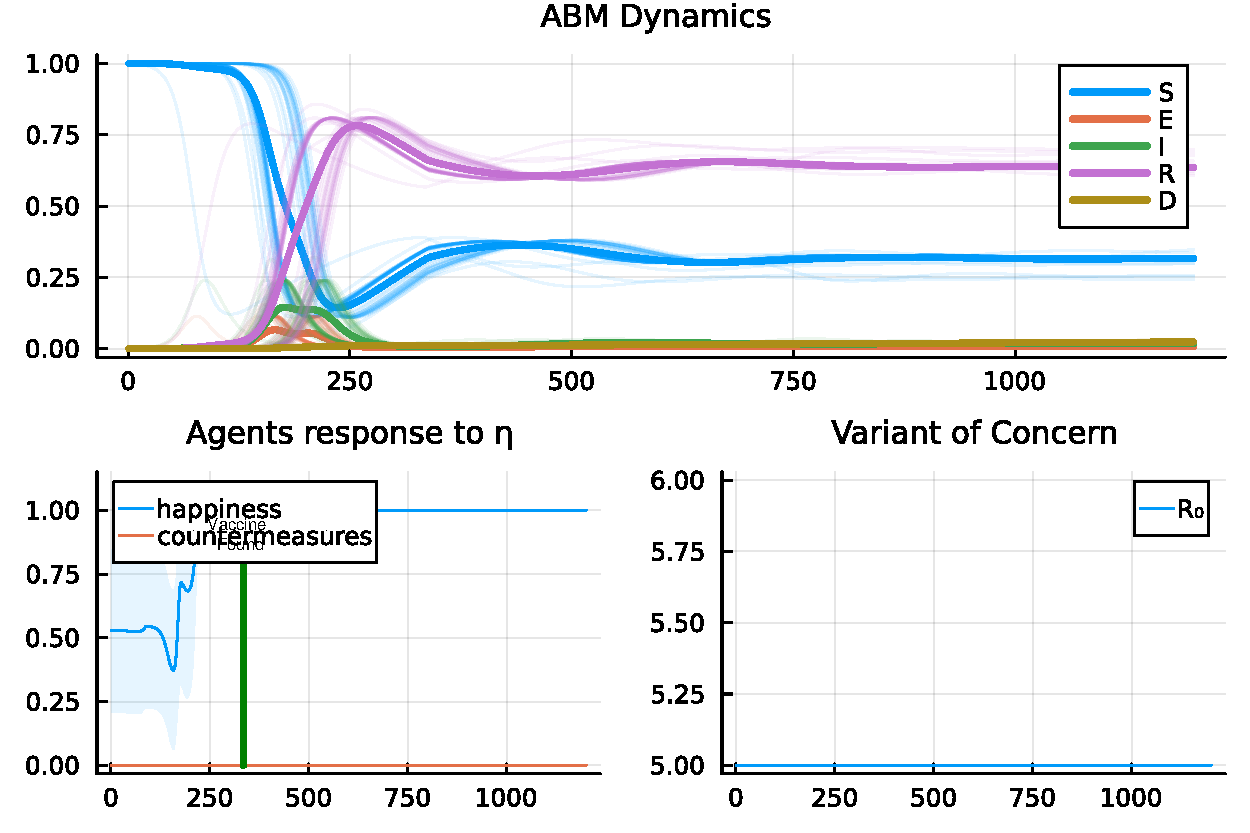
\includegraphics[width=\textwidth]{img/SocialNetworkABM_5_V.pdf}
		\caption{Grafico per la comparazione sul periodo di inizio della campagna vaccinale. Poco dopo la prima ondata}
		\label{fig:comparison_vax_3}
	\end{subfigure}
	\hfill
	\begin{subfigure}[b]{0.45\textwidth}
		\centering
		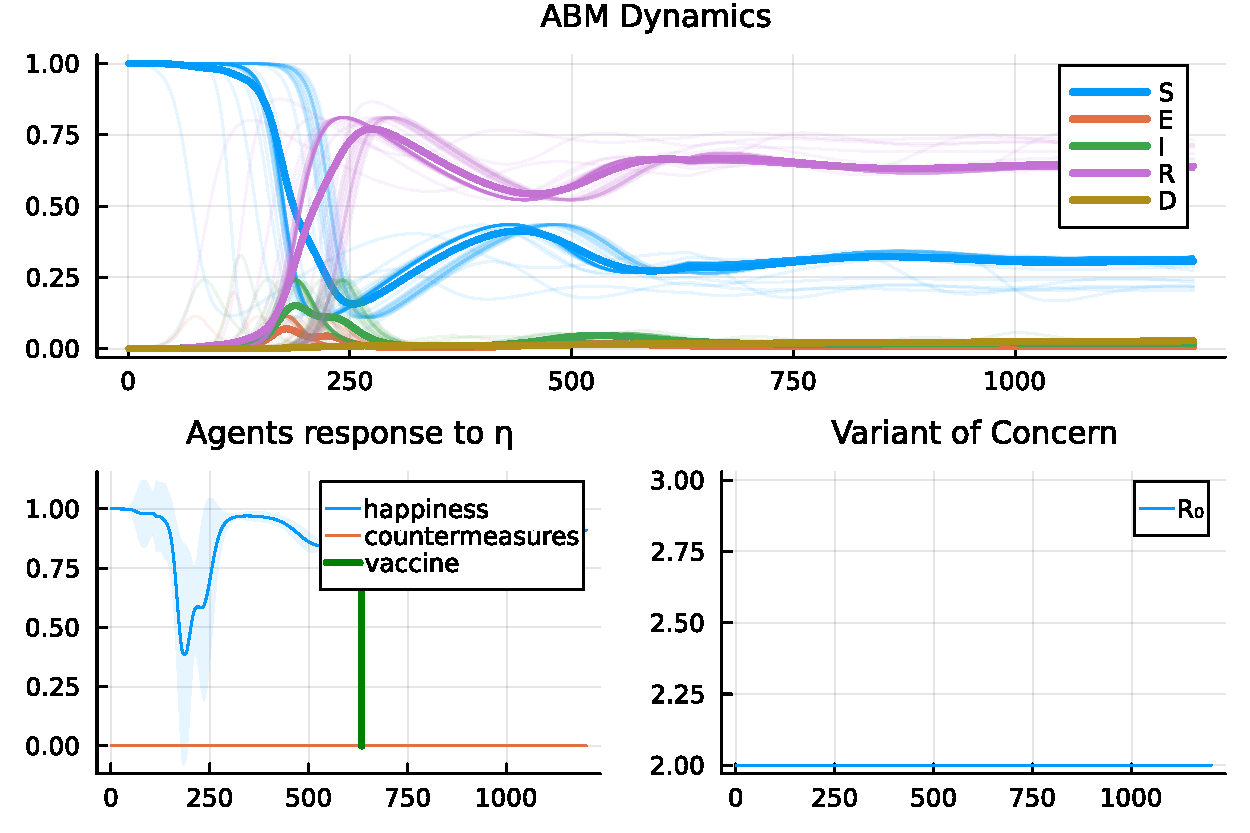
\includegraphics[width=\textwidth]{img/SocialNetworkABM_2_V.pdf}
		\caption{Grafico per la comparazione sul periodo di inizio della campagna vaccinale. In ritardo}
		\label{fig:comparison_vax_4}
	\end{subfigure}
\end{figure}

\subsection{Intervento Farmaceutico e Non Farmaceutico}

Il seguente grafico (Figura \ref{fig:abm_combined_intervent}) 
rappresenta l'andamento delle curve quando vengono applicati sia 
un intervento farmaceutico che un intervento non farmaceutico. 
L'obiettivo di questa combinazione di interventi è quello di 
massimizzare la riduzione della diffusione del virus e di contenere 
l'epidemia in modo ottimale.

\begin{minipage}{\linewidth}
    \centering
    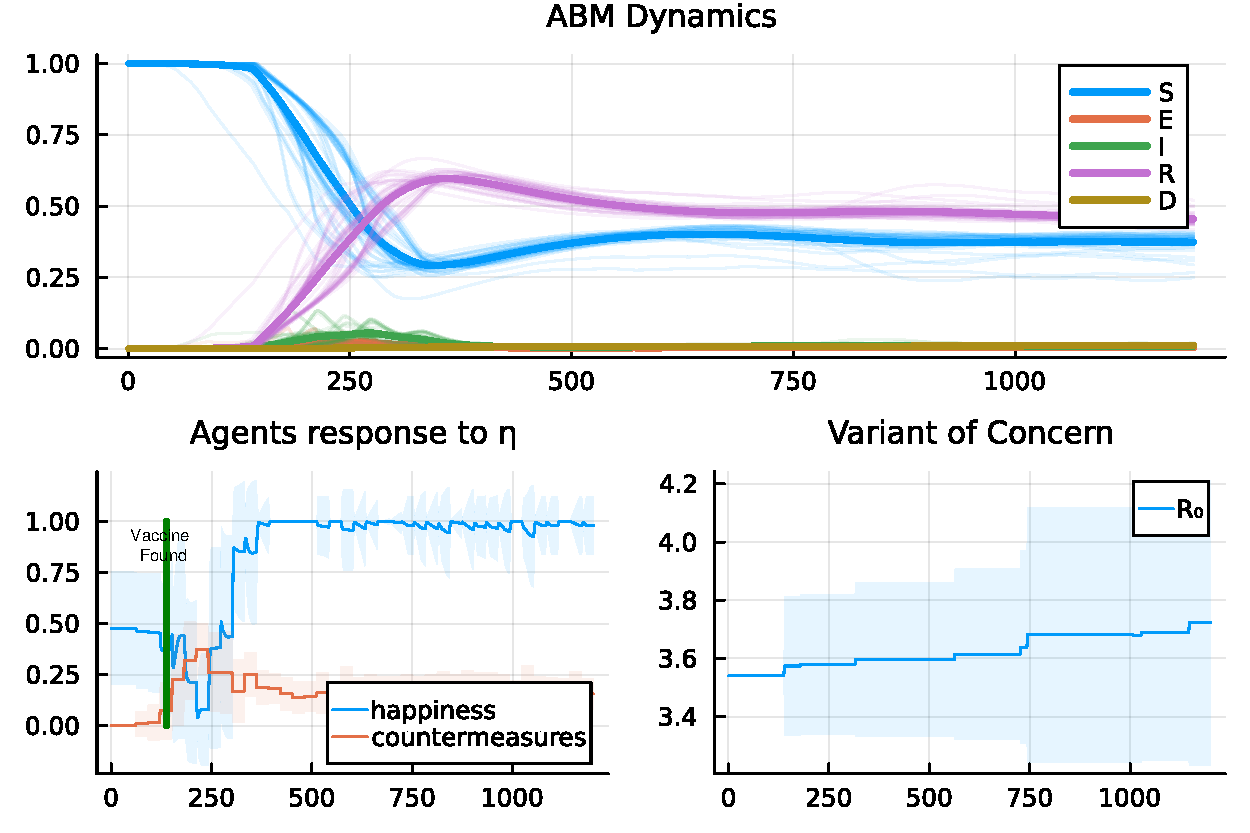
\includegraphics[width=\textwidth]{img/SocialNetworkABM_ALL.pdf}
    \captionof{figure}{Grafico cumulativo del modello con intervento farmaceutico e non farmaceutico combinato}
    \label{fig:abm_combined_intervent}
\end{minipage}

Come mostrato nel grafico, l'effetto combinato di intervento 
farmaceutico e non farmaceutico è estremamente efficace nel 
contenere l'epidemia. Il numero di individui suscettibili 
rimane stabile nel tempo, e l'epidemia viene rapidamente ridotta 
a livelli molto bassi. La curva di individui guariti mostra un 
aumento costante nel tempo, poiché l'intervento farmaceutico 
garantisce immunità duratura.

La curva di felicità mostra ancora alcune oscillazioni dovute 
alle misure di controllo cicliche, ma queste oscillazioni sono 
molto meno pronunciate rispetto ai casi precedenti.

In generale, la combinazione di intervento farmaceutico e non 
farmaceutico è altamente efficace nel contenere e ridurre 
l'epidemia in modo ottimale.
\newpage

\subsubsection{Grafici di Confronto}

I grafici di confronto mostrano l'impatto del momento di inizio della 
campagna di vaccinazione su diversi scenari. Questi grafici illustrano 
come l'efficacia della campagna vaccinale possa dipendere dal suo avvio, 
oltre al numero di persone vaccinate, e come questa influenzi attivamente
le contromisure non farmaceutiche.

\begin{figure}[!hb]
	\centering
	\begin{subfigure}[b]{0.45\textwidth}
		\centering
		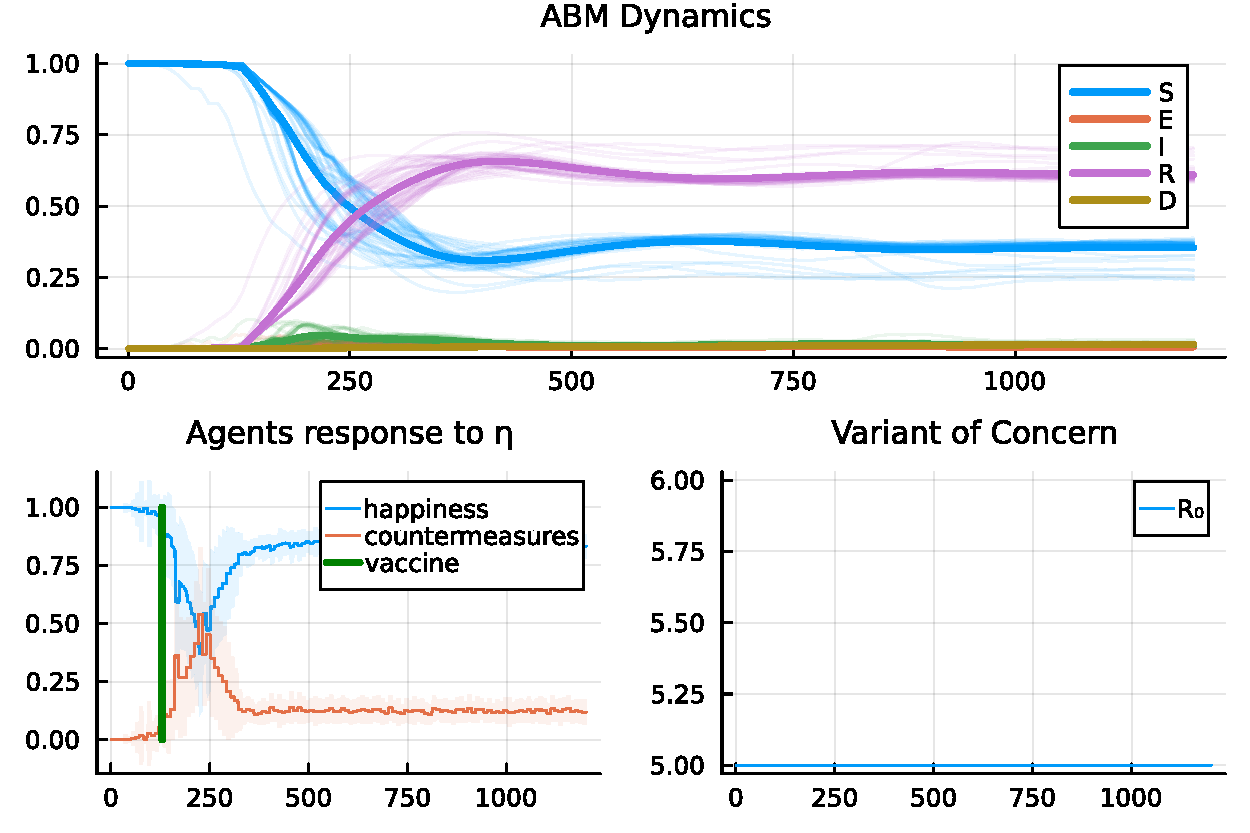
\includegraphics[width=\textwidth]{img/SocialNetworkABM_5_A.pdf}
		\caption{Grafico per la comparazione sul periodo di inizio della campagna vaccinale. Immediata}
		\label{fig:comparison_all_1}
	\end{subfigure}
	\hfill
	\begin{subfigure}[b]{0.45\textwidth}
		\centering
		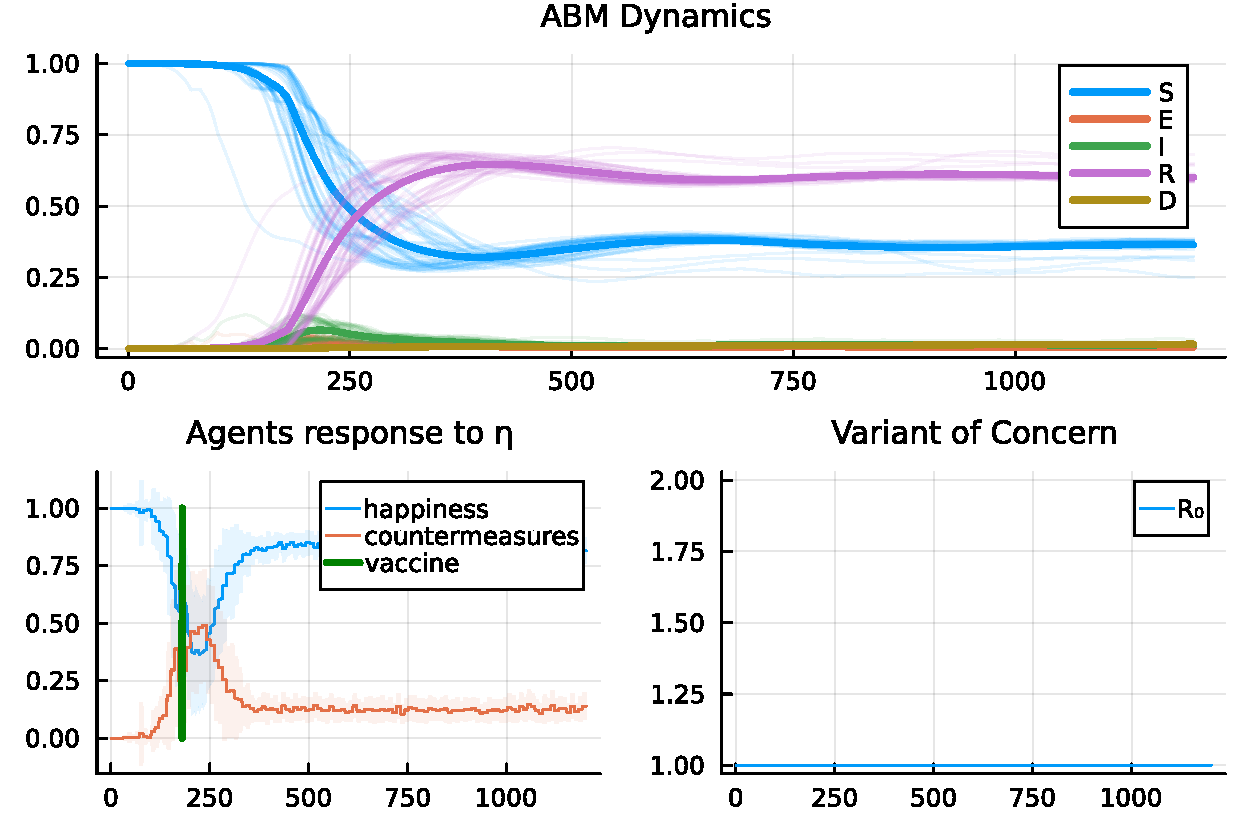
\includegraphics[width=\textwidth]{img/SocialNetworkABM_1_A.pdf}
		\caption{Grafico per la comparazione sul periodo di inizio della campagna vaccinale. Durante prima ondata}
		\label{fig:comparison_all_2}
	\end{subfigure}
	\hfill
	\begin{subfigure}[b]{0.45\textwidth}
		\centering
		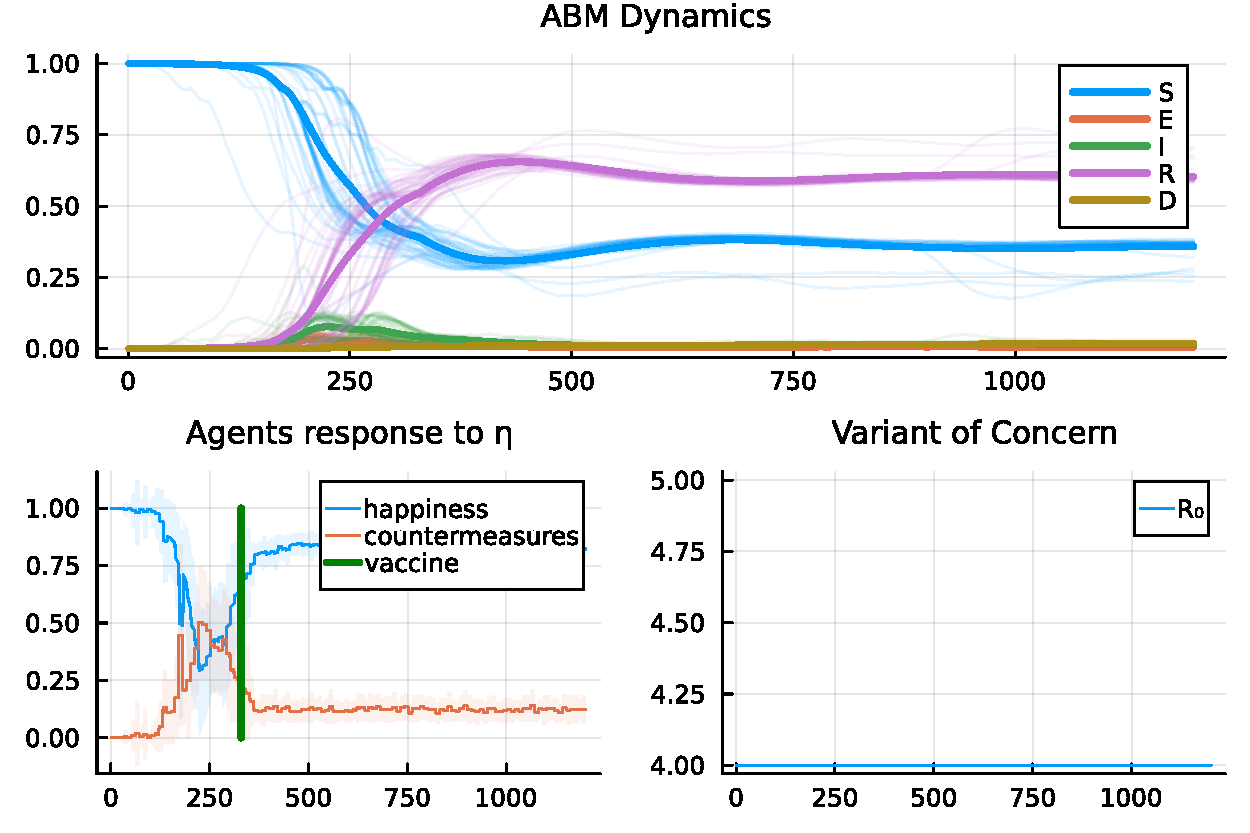
\includegraphics[width=\textwidth]{img/SocialNetworkABM_4_A.pdf}
		\caption{Grafico per la comparazione sul periodo di inizio della campagna vaccinale. Poco dopo la prima ondata}
		\label{fig:comparison_all_3}
	\end{subfigure}
	\hfill
	\begin{subfigure}[b]{0.45\textwidth}
		\centering
		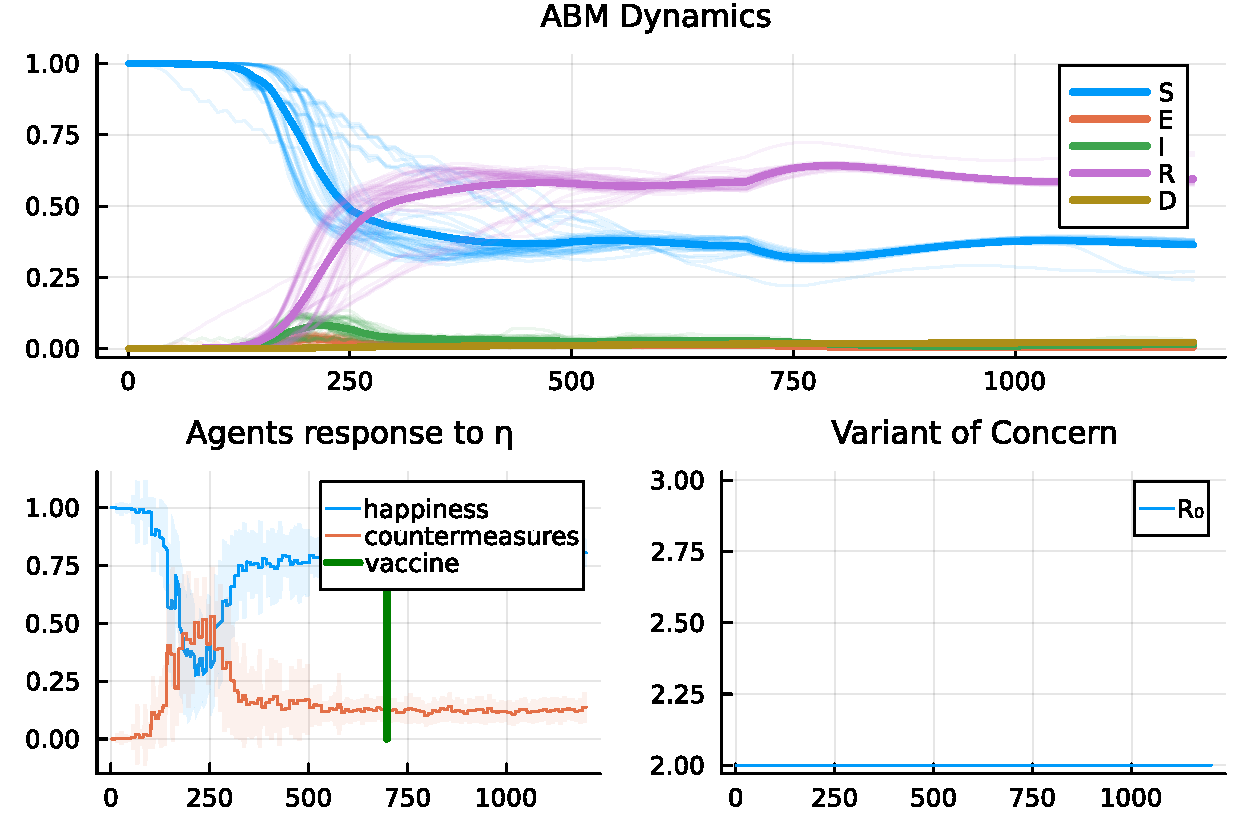
\includegraphics[width=\textwidth]{img/SocialNetworkABM_2_A.pdf}
		\caption{Grafico per la comparazione sul periodo di inizio della campagna vaccinale. In ritardo}
		\label{fig:comparison_all_4}
	\end{subfigure}
\end{figure}
\newpage

\section{Conclusioni}

In conclusione, i risultati ottenuti dimostrano chiaramente 
l'efficacia delle misure di controllo, sia farmaceutiche che non 
farmaceutiche, nel contenere e ridurre la diffusione del virus. 
L'intervento farmaceutico, in particolare, si è dimostrato altamente 
efficace nel contrastare l'epidemia e nel prevenire il ciclo 
insostenibile di infezioni. Tuttavia, è importante sottolineare che 
l'intervento farmaceutico da solo potrebbe non essere sufficiente per 
l'eliminazione completa dell'epidemia. Al contrario, l'adozione di una 
combinazione di interventi farmaceutici e non farmaceutici offre una 
protezione ottimale e una strategia più completa per la gestione delle 
pandemie.

Va notato che i tempi di calcolo delle simulazioni sono notevolmente 
influenzati dall'applicazione delle misure di controllo non farmaceutiche. 
Tuttavia, questa è una compromissione necessaria per ottenere risultati 
accurati e realistici che tengano conto della complessità delle dinamiche 
sociali ed epidemiologiche. Inoltre, l'osservazione di oscillazioni 
nelle curve di felicità, causate dall'uso di misure di controllo cicliche, 
non rappresenta un problema insormontabile e può essere gestita 
adeguatamente.

In generale, il modello di simulazione dell'epidemia su una rete sociale 
si configura come una piattaforma estremamente utile per lo studio degli 
effetti delle misure di controllo e per lo sviluppo di strategie ottimali 
per la gestione delle epidemie. I risultati ottenuti contribuiscono alla 
comprensione e alla preparazione per affrontare situazioni 
epidemiologiche complesse e dinamiche come quelle delle pandemie.